\section{Use Case: Coordination of the Heterogeneous Model of a Surveillance Camera System}
This section presents the heterogeneous model of a surveillance camera system (Figure~\ref{fig:camerasystem}). To model different parts of the system, we use the TFSM and Activity languages. In the following, we first present the different subsystems, and then, we propose a set of coordination pattern to coordinate the behavior of the different models. 

The video surveillance system is composed of a camera and a battery control. The camera takes pictures by using either the \emph{JPEG2000} or \emph{JPG} algorithm and is powered by a battery. Roughly speaking, the JPEG\footnote{http://www.jpeg.org} algorithm encodes a picture by grouping it in blocks which are transformed by a \textit{forward transformation}. Each block of pixels is transformed to frequency coefficient using either a \textit{Fourier transform} (JPEG) or \textit{Wavelet transform} (JPEG2000). The transformed blocks are \textit{quantized} and then passed to a \textit{Run-Length coder} which compress the data. At the end, the block is \textit{transmitted}. In the camera, when the battery is low, the battery control makes the camera use the \emph{JPG} algorithm, thus reducing the quality of the picture but also the energy consumption~\cite{encodingcomparison}. When the battery is high, the JPEG2000 algorithm is used instead. 

Figure~\ref{fig:camerasystem} shows the whole model of the camera system. At the top of Figure, the activity diagrams named \emph{BatteryControl} represents the simple algorithm implemented in the battery control. Depending on the status of the battery, the algorithm executes either the action \emph{BatteryisLow} or \emph{BatteryisHigh}, which correspond with the occurrence of the \mse \emph{BatteryisLow:executeIt} and \emph{BatteryisHigh:executeIt} respectively. At the bottom of Figure~\ref{fig:camerasystem}, the TFSM named \emph{CameraControl} represents a partial view of the camera. When the TFSM model is in state \emph{BatteryHigh}, the JPEG2000 algorithm is used (specified by the activity diagram on the right of Figure~\ref{fig:camerasystem} named \emph{doJPEG2000}). When in state \emph{BatteryLow}, the encoding algorithm is replaced by a mere JPEG algorithm represented by an activity named \emph{doJPEG}. The transition from one state to another is done when either the \emph{BatteryisHigh:occurs} event or the \emph{BatteryisLow:occurs} event occurs, depending on the current state.	   

\begin{figure}
	\center
	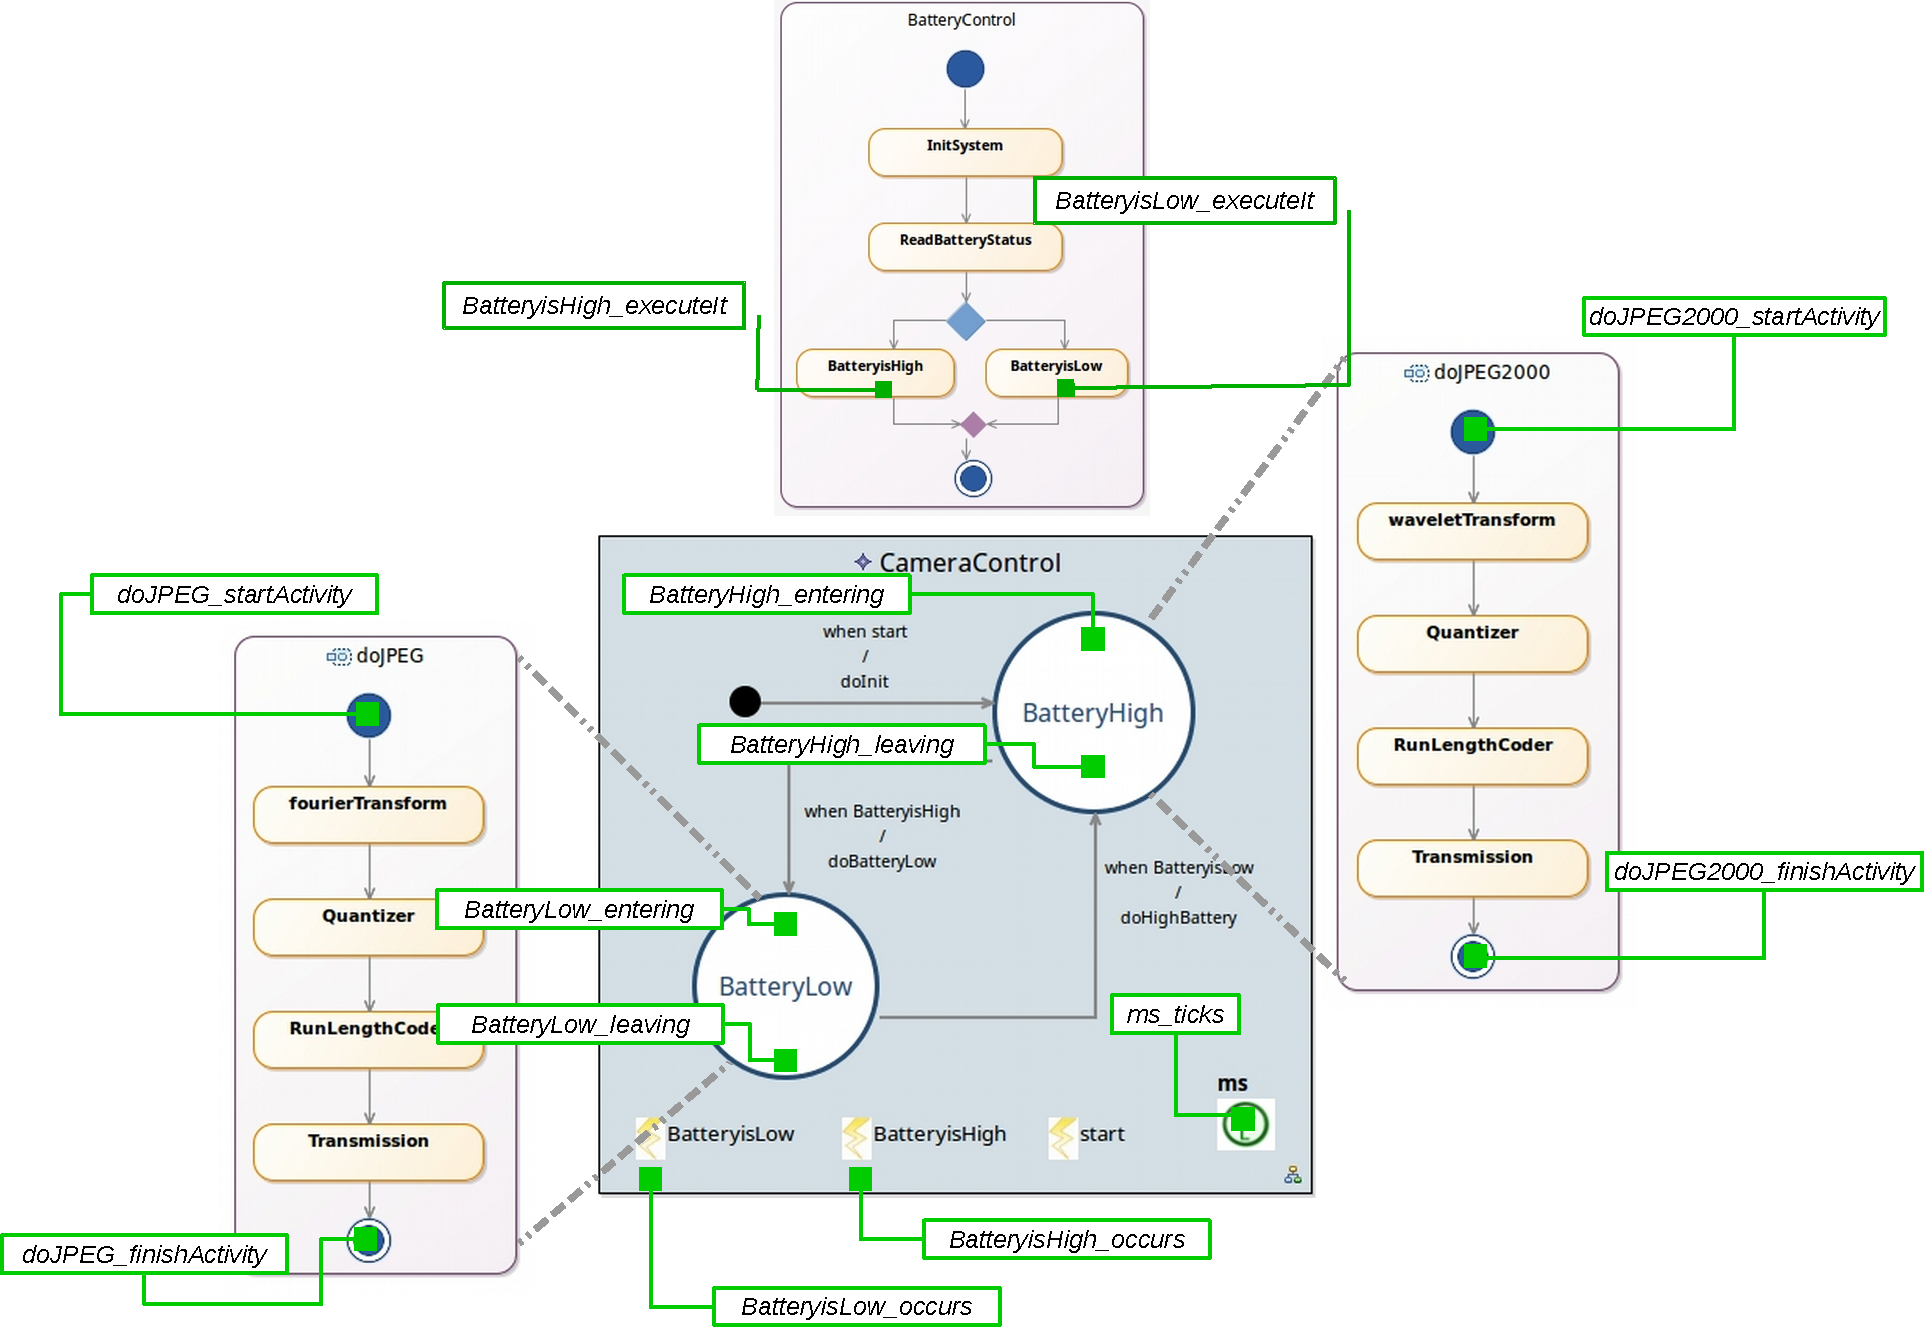
\includegraphics[width=1\columnwidth]{examples/figs/picmodels.pdf}
	\caption{Hierarchical model of a surveillance camera system and a partial representation of the behavioral interface}
	\label{fig:camerasystem}
\end{figure}

To represent the global behavior of the surveillance camera system, we have to specify how these models are coordinated. To do so, we propose a set of coordination patterns between the TFSM and Activity languages. In the following, we present the models that must be coordinated together with the pattern to coordinate them. 

The activity BatteryControl and the TFSM CameraControl are coordinated by relying on Actions and FSMEvents. More precisely, the execution of the actions \emph{BatteryisHigh} and \emph{BatteryisLow} must be synchronized with the occurrences of the FSMEvents \emph{BetteryisHigh} and \emph{BatteryisLow}, \ie synchronization between the \mse \emph{BatteryisHigh:executeIt} and \emph{BatteryisHigh:occurs}, and the \mse \emph{BatteryisLow:executeIt} and \emph{BatteryisLow:occurs}. Thus, to coordinate the BatteryControl and the CameraControl, we propose to reuse the operator \emph{SyncFSMEventsAndActions} (see Listing~\ref{lst:bcoolrunningexample}: line 5), which coordinates instances of \dse \emph{occurs} and instances \dse \emph{executeIt} by relying on their names. 

In addition, the execution of the states of the TFSM CameraControl must be coordinated with the activities doJPEG and doJPEG2000. To coordinate these models, we have to coordinate the entering and leaving of a state and the execution of the activities. In this example, we chose the semantics in which entering a specific state of a TFSM model triggers the execution of a given Activity. Then, when leaving a state, several semantic variation points may be chosen. The outgoing transitions from a state can be considered, for instance, as preemptive for the activity model (\ie firing a transition from a state to another preempts the internal activity). Alternatively, the transition can be considered as non-preemptive (\ie the states cannot be left before the associated activity finishes). In our case, we chose non-preemptive transitions. This results that, when the states are reached, the corresponding activity is executed. Then, the state can be left only if the activity has finished. To capture the specification of this coordination pattern, we propose to define a \bcool operator named \emph{startActivityWhenEnter} that implements a hierarchical coordination between states and activity in which transition are non-preemptive.     

Together with the operator \emph{startActivityWhenEnter}, we propose to specify how the time in the TFSM elapses during the execution of activities. We propose a coordination pattern to coordinate the time between the TFSM and Activity languages. In these languages, the time is represented differently. In the TFSM language, each state machine has a \emph{localClock} used to measure the time while the Activity language is untimed. The local clock is a \emph{FSMClock}, which defines a \dse named \emph{ticks} whose occurrences represent a physical time increment. In the Activity language, the duration of activities can be represented as the time between the \dse \emph{startActivity} and \dse \emph{finishActivity}. Thus, to coordinate the time, it is necessary to specify the number of \emph{ticks} of the local clock between the occurrence of the \dse \emph{startActivity} and \emph{finishActivity}. We propose to enforce the execution of the ``internal'' activity to be atomic with respect to the time in the TFSM model. As a result, there are no occurrences of the \dse ticks of the corresponding local clock during the execution of the activity. For example, in the camera, this would result in no occurrences of the \mse \emph{ms:ticks} between the occurrences of the \mse \emph{doJPEG2000:startActivity}, \emph{doJPEG2000:finishActivity}. To capture the specification of this coordination pattern, we propose to define a \bcool operator named \emph{AtomicActivity}, which is also hierarchical but only considers timing aspects.   


In this section, we have presented the model of a surveillance camera system. To model the system, we used TFSM and Activity languages thus resulting in a heterogeneous model. To coordinate these models, we have described three coordination patterns between the TFSM and Activity languages and we have proposed three \bcool operator to capture their specification:
	\begin{itemize}
		\item \emph{SyncFSMEventsAndActions}, which specifies a coordination pattern that coordinates Actions and FSMEvents;
		\item \emph{startActivityWhenEnter}, which specifies a hierarchical coordination pattern that coordinates the entering and leaving of states and the execution of Activities; 
		\item \emph{AtomicActivity}, which specifies a coordination pattern that coordinates the time between TFSMs and Activities. 
	\end{itemize}
	
In the following section, we specify these operators in \bcool. For the operator \emph{SyncFSMEventsAndActions}, we rely on the specification presented in chapter~\ref{ch:bcool}. 
